\documentclass{article}
    % General document formatting
    \usepackage[margin=0.7in]{geometry}
    \usepackage[parfill]{parskip}
    \usepackage[utf8]{inputenc}
    \usepackage{amsmath}
    \usepackage{amssymb}
    \usepackage{tikz}
    \usepackage{fancyhdr}
    \usepackage{listings}
    \usepackage{multicol}
    \usepackage{polynom}

\pagestyle{fancy}
\fancyhf{}
\rhead{Edgar Jacob Rivera Rios - A01184125}

\begin{document}
\begin{titlepage}

    \newcommand{\HRule}{\rule{\linewidth}{0.5mm}} % Defines a new command for the horizontal lines, change thickness here

    \center % Center everything on the page

    %----------------------------------------------------------------------------------------
    %	HEADING SECTIONS
    %----------------------------------------------------------------------------------------

    \textsc{\LARGE Tecnológico de Monterrey}\\[1.5cm] % Name of your university/college
    \textsc{\Large Fundamentos de computación}\\[0.5cm] % Major heading such as course name
    %\textsc{\large Minor Heading}\\[0.5cm] % Minor heading such as course title

    %----------------------------------------------------------------------------------------
    %	TITLE SECTION
    %----------------------------------------------------------------------------------------

    \HRule \\[0.4cm]
    { \huge \bfseries Homework 7}\\[0.4cm] % Title of your document
    \HRule \\[1.5cm]

    %----------------------------------------------------------------------------------------
    %	AUTHOR SECTION
    %----------------------------------------------------------------------------------------

    \begin{minipage}{0.4\textwidth}
    \begin{flushleft} \large
    \emph{Student:}\\
    Jacob \textsc{Rivera} % Your name
    \end{flushleft}
    \end{minipage}
    ~
    \begin{minipage}{0.4\textwidth}
    \begin{flushright} \large
    \emph{Professor:} \\
    Dr. Hugo \textsc{Terashima} % Supervisor's Name
    \end{flushright}
    \end{minipage}\\[2cm]

    % If you don't want a supervisor, uncomment the two lines below and remove the section above
    %\Large \emph{Author:}\\
    %John \textsc{Smith}\\[3cm] % Your name

    %----------------------------------------------------------------------------------------
    %	DATE SECTION
    %----------------------------------------------------------------------------------------

    {\large \today}\\[2cm] % Date, change the \today to a set date if you want to be precise

    %----------------------------------------------------------------------------------------
    %	LOGO SECTION
    %----------------------------------------------------------------------------------------

    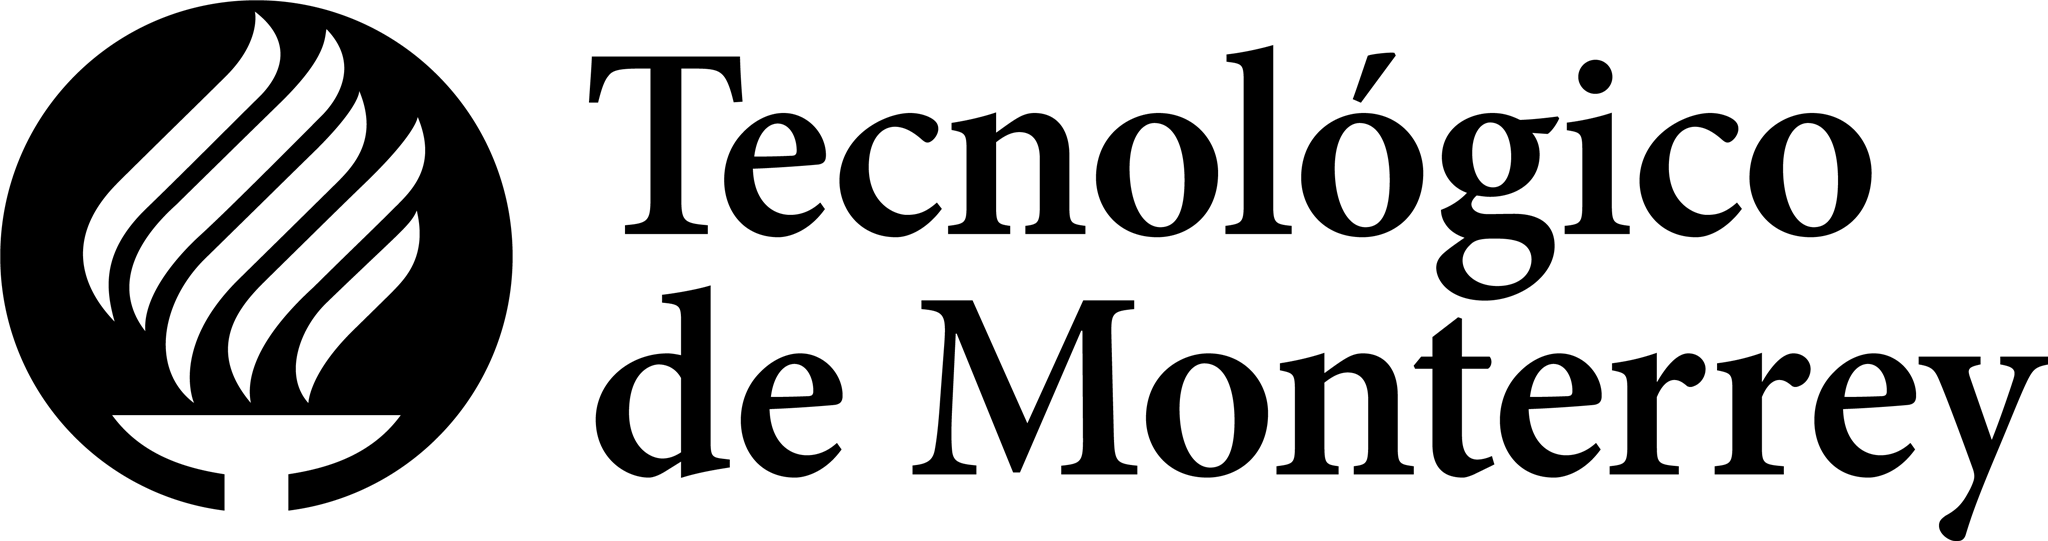
\includegraphics[width=0.4\textwidth,height=\textheight,keepaspectratio]{logo-tec-negro.png} % Include a department/university logo - this will require the graphicx package

    %----------------------------------------------------------------------------------------

    \vfill % Fill the rest of the page with whitespace

\end{titlepage}


\section{Problems}
Solve the following problems:
\begin{enumerate}
    \item Generate two 4 X 4 matrices and manually apply the Strassen’s method to multiply them. Verify that the result is correct by comparing with the one provided by the traditional method. Show the steps.
    \begin{multicols}{2}
        \begin{center}
            $A=$
            \begin{tabular}{|c c c c|}
                \hline
                1&2&3&4\\
                5&6&7&8\\
                9&10&11&12\\
                13&14&15&16\\
                \hline
            \end{tabular}\\
            $B=$
            \begin{tabular}{|c c c c|}
                \hline
                16&15&14&13\\
                12&11&10&9\\
                8&7&6&5\\
                4&3&2&1\\
                \hline
            \end{tabular}
        \end{center}
    \end{multicols}
    \begin{multicols}{2}
        \begin{center}
            $A=$
            \begin{tabular}{|c c|c c|}
                \hline
                1&2&3&4\\
                5&6&7&8\\
                \hline
                9&10&11&12\\
                13&14&15&16\\
                \hline
            \end{tabular}\\
            $B=$
            \begin{tabular}{|c c|c c|}
                \hline
                16&15&14&13\\
                12&11&10&9\\
                \hline
                8&7&6&5\\
                4&3&2&1\\
                \hline
            \end{tabular}
        \end{center}
    \end{multicols}
    \begin{multicols}{4}
        \begin{center}
            $A_1=$
            \begin{tabular}{|c c|}
                \hline
                1&2\\
                5&6\\
                \hline
            \end{tabular}\\
            $A_3=$
            \begin{tabular}{|c c|}
                \hline
                9&10\\
                13&14\\
                \hline
            \end{tabular}\\
            $A_2=$
            \begin{tabular}{|c c|}
                \hline
                3&4\\
                7&8\\
                \hline
            \end{tabular}\\
            $A_4=$
            \begin{tabular}{|c c|}
                \hline
                11&12\\
                15&16\\
                \hline
            \end{tabular}\\
            $B_1=$
            \begin{tabular}{|c c|}
                \hline
                16&15\\
                12&11\\
                \hline
            \end{tabular}\\
            $B_3=$
            \begin{tabular}{|c c|}
                \hline
                8&7\\
                4&3\\
                \hline
            \end{tabular}\\
            $B_2=$
            \begin{tabular}{|c c|}
                \hline
                14&13\\
                10&9\\
                \hline
            \end{tabular}\\
            $B_4=$
            \begin{tabular}{|c c|}
                \hline
                6&5\\
                2&1\\
                \hline
            \end{tabular}\\
        \end{center}
    \end{multicols}

    \begin{align*}
        C_1 &= A_1  B_1\\
        C_2 &= A_2  B_2\\
        C_3 &= A_3  B_3\\
        C_4 &= A_4  B_4
    \end{align*}

    \begin{multicols}{2}
        \begin{center}
            $A_1B_1$\\
            \begin{align*}
                X_1 &= (1 + 6) * (16 + 11) = 189\\
                X_2 &= 16 * (5 + 6) = 176\\
                X_3 &= 1 * (15-11) = 4 \\
                X_4 &= 6 * (12 - 16) = -24\\
                X_5 &= 11 * (1 + 2) = 33\\
                X_6 &= (5 - 1) * (16 + 15) = 124\\
                X_7 &= (2 - 6) * (12 + 11) = -92\\
            \end{align*}
            $C_1=$
            \begin{tabular}{|c c|}
                \hline
                189 + -24 - 33 + -92 &4 + 33\\
                176 + -24& 189 + 4 - 176 + 124\\
                \hline
            \end{tabular}\\
            $=$
            \begin{tabular}{|c c|}
                \hline
                40&37\\
                152&141\\
                \hline
            \end{tabular}\\
        \end{center}

        \begin{center}
            $A_2B_2$\\
            \begin{align*}
                X_1 &= (3 + 8) * (14 + 9) = 253\\
                X_2 &= 14 * (7 + 8) = 210\\
                X_3 &= 3 * (13-9) = 12 \\
                X_4 &= 8 * (10 - 14) = -32\\
                X_5 &= 9 * (3 + 4) = 63 \\
                X_6 &= (7 - 3) * (14 + 13) = 108\\
                X_7 &= (4 - 8) * (10 + 9) = -76\\
            \end{align*}
            $C_2=$
            \begin{tabular}{|c c|}
                \hline
                253 + -32 - 63 + -76 &12 + 63\\
                210 + -32& 253 + 12 - 210 + 108\\
                \hline
            \end{tabular}\\
            $=$
            \begin{tabular}{|c c|}
                \hline
                82&75\\
                178&163\\
                \hline
            \end{tabular}\\
        \end{center}
    \end{multicols}
    \pagebreak
    \begin{multicols}{2}
        \begin{center}
            $A_3B_3$\\
            \begin{align*}
                X_1 &= (3 + 8) * (14 + 9)  = 253\\
                X_2 &= 8 * (13 + 14) = 216\\
                X_3 &= 9 * (7 -3) = 36 \\
                X_4 &= 14 * (4 - 8) = -56\\
                X_5 &= 3 * (9 + 10) = 57\\
                X_6 &= (13 - 9) * (8 + 7) = 60\\
                X_7 &= (10 - 14) * (4 + 3) = -28\\
            \end{align*}
            $C_3=$
            \begin{tabular}{|c c|}
                \hline
                253 + -56 - 57 + -28 &36 + 57\\
                216 + -56& 253 + 36 - 216 + 60\\
                \hline
            \end{tabular}\\
            $=$
            \begin{tabular}{|c c|}
                \hline
                112&93\\
                160&133\\
                \hline
            \end{tabular}\\
        \end{center}

        \begin{center}
            $A_4B_4$\\
            \begin{align*}
                X_1 &= (1 + 6) * (16 + 11) = 189\\
                X_2 &= 6 * (15 + 16) = 186\\
                X_3 &= 11 * (5-1) = 44\\
                X_4 &= 16 * (2 - 6) = -64\\
                X_5 &= 1 * (11 + 12) = 23 \\
                X_6 &= (15 - 11) * (6 + 5) = 44\\
                X_7 &= (12 - 16) * (2 + 1) = -12\\
            \end{align*}
            $C_4=$
            \begin{tabular}{|c c|}
                \hline
                189 + -64 - 23 + -12 &44 + 23\\
                186 + -64& 189 + 44 - 186 + 44\\
                \hline
            \end{tabular}\\
            $=$
            \begin{tabular}{|c c|}
                \hline
                90&67\\
                122&91\\
                \hline
            \end{tabular}\\
        \end{center}
    \end{multicols}

    \item Generate a monic polynomial with $k= 4$ (that is $n= 15$) and solve it using the recursive algorithm presented in class. show the steps.
    \begin{equation*}
        x^{15}+2x^{14}+3x^{13}+4x^{12}+x^{11}+2x^{10}+3x^{9}+4x^{8}+x^{7}+2x^{6}+3x^{5}+4x^{4}+x^{3}+2x^{2}+3x+4
    \end{equation*}
    \begin{align*}
        k &= 4\\
        j &= 2^{k-1} = 8\\
        b &= a_{2^{k-1}-1} - 1 = a_7 - 1 = 0
    \end{align*}
    *\[\polylongdiv{x^{15}+2x^{14}+3x^{13}+4x^{12}+x^{11}+2x^{10}+3x^{9}+4x^{8}+x^{7}+2x^{6}+3x^{5}+4x^{4}+x^{3}+2x^{2}+3x+4}{x^8}\]

    \begin{equation*}
        p(x) = (x^8)(x^7+ 2x^6+ 3x^5+ 4x^4+x^3+ 2x^2+ 3x+ 4) + (x^7+ 2x^6+ 3x^5+ 4x^4+x^3+ 2x^2+ 3x+ 4)
    \end{equation*}

    \begin{equation*}
        x^7+ 2x^6+ 3x^5+ 4x^4+x^3+ 2x^2+ 3x+ 4
    \end{equation*}
    \begin{align*}
        k &= 3\\
        j &= 2^{k-1} = 4\\
        b &= a_{2^{k-1}-1} - 1 = a_3 - 1 = 0
    \end{align*}
    *\[\polylongdiv{x^7+ 2x^6+ 3x^5+ 4x^4+x^3+ 2x^2+ 3x+ 4}{x^4}\]

    \begin{equation*}
        p(x) = (x^8)((x^4)(x^3+ 2x^2+ 3x+ 4) + (x^3+ 2x^2+ 3x+ 4)) + (x^7+ 2x^6+ 3x^5+ 4x^4+x^3+ 2x^2+ 3x+ 4)
    \end{equation*}

    \begin{equation*}
        x^3+ 2x^2+ 3x+ 4
    \end{equation*}
    \begin{align*}
        k &= 2\\
        j &= 2^{k-1} = 2\\
        b &= a_{2^{k-1}-1} - 1 = a_1 - 1 = 3
    \end{align*}
    *\[\polylongdiv{x^3+ 2x^2+ 3x+ 4}{x^2+3}\]

    \begin{equation*}
        p(x) = (x^8)((x^4)((x^2 +3)(x+ 2) + (-2)) + (x^3+ 2x^2+ 3x+ 4)) + (x^7+ 2x^6+ 3x^5+ 4x^4+x^3+ 2x^2+ 3x+ 4)
    \end{equation*}

    \begin{equation*}
        p(x) = (x^8)[(x^4)((x^2 +3)(x+ 2) + -2) + (x^2 +3)(x+ 2) + -2] + [(x^4)((x^2 +3)(x+ 2) + -2) + (x^2 +3)(x+ 2) + -2]
    \end{equation*}
    \begin{equation*}
        p(x) = (x^8)[(x^4)((x^2 +3)(x+ 2) + -2) + (x^2 +3)(x+ 2) + -2] + (x^4)((x^2 +3)(x+ 2) + -2) + (x^2 +3)(x+ 2) + -2
    \end{equation*}

\end{enumerate}
\end{document}